% Options for packages loaded elsewhere
\PassOptionsToPackage{unicode}{hyperref}
\PassOptionsToPackage{hyphens}{url}
%
\documentclass[
  ignorenonframetext,
]{beamer}
\usepackage{pgfpages}
\setbeamertemplate{caption}[numbered]
\setbeamertemplate{caption label separator}{: }
\setbeamercolor{caption name}{fg=normal text.fg}
\beamertemplatenavigationsymbolsempty
% Prevent slide breaks in the middle of a paragraph
\widowpenalties 1 10000
\raggedbottom
\setbeamertemplate{part page}{
  \centering
  \begin{beamercolorbox}[sep=16pt,center]{part title}
    \usebeamerfont{part title}\insertpart\par
  \end{beamercolorbox}
}
\setbeamertemplate{section page}{
  \centering
  \begin{beamercolorbox}[sep=12pt,center]{part title}
    \usebeamerfont{section title}\insertsection\par
  \end{beamercolorbox}
}
\setbeamertemplate{subsection page}{
  \centering
  \begin{beamercolorbox}[sep=8pt,center]{part title}
    \usebeamerfont{subsection title}\insertsubsection\par
  \end{beamercolorbox}
}
\AtBeginPart{
  \frame{\partpage}
}
\AtBeginSection{
  \ifbibliography
  \else
    \frame{\sectionpage}
  \fi
}
\AtBeginSubsection{
  \frame{\subsectionpage}
}
\usepackage{amsmath,amssymb}
\usepackage{lmodern}
\usepackage{ifxetex,ifluatex}
\ifnum 0\ifxetex 1\fi\ifluatex 1\fi=0 % if pdftex
  \usepackage[T1]{fontenc}
  \usepackage[utf8]{inputenc}
  \usepackage{textcomp} % provide euro and other symbols
\else % if luatex or xetex
  \usepackage{unicode-math}
  \defaultfontfeatures{Scale=MatchLowercase}
  \defaultfontfeatures[\rmfamily]{Ligatures=TeX,Scale=1}
\fi
\usetheme[]{Warsaw}
% Use upquote if available, for straight quotes in verbatim environments
\IfFileExists{upquote.sty}{\usepackage{upquote}}{}
\IfFileExists{microtype.sty}{% use microtype if available
  \usepackage[]{microtype}
  \UseMicrotypeSet[protrusion]{basicmath} % disable protrusion for tt fonts
}{}
\makeatletter
\@ifundefined{KOMAClassName}{% if non-KOMA class
  \IfFileExists{parskip.sty}{%
    \usepackage{parskip}
  }{% else
    \setlength{\parindent}{0pt}
    \setlength{\parskip}{6pt plus 2pt minus 1pt}}
}{% if KOMA class
  \KOMAoptions{parskip=half}}
\makeatother
\usepackage{xcolor}
\IfFileExists{xurl.sty}{\usepackage{xurl}}{} % add URL line breaks if available
\IfFileExists{bookmark.sty}{\usepackage{bookmark}}{\usepackage{hyperref}}
\hypersetup{
  pdftitle={Introduction to R and RStudio},
  pdfauthor={Stephen Roecker, Skye Wills, Katey Yoast and Tom D'Avello},
  hidelinks,
  pdfcreator={LaTeX via pandoc}}
\urlstyle{same} % disable monospaced font for URLs
\newif\ifbibliography
\usepackage{color}
\usepackage{fancyvrb}
\newcommand{\VerbBar}{|}
\newcommand{\VERB}{\Verb[commandchars=\\\{\}]}
\DefineVerbatimEnvironment{Highlighting}{Verbatim}{commandchars=\\\{\}}
% Add ',fontsize=\small' for more characters per line
\usepackage{framed}
\definecolor{shadecolor}{RGB}{248,248,248}
\newenvironment{Shaded}{\begin{snugshade}}{\end{snugshade}}
\newcommand{\AlertTok}[1]{\textcolor[rgb]{0.94,0.16,0.16}{#1}}
\newcommand{\AnnotationTok}[1]{\textcolor[rgb]{0.56,0.35,0.01}{\textbf{\textit{#1}}}}
\newcommand{\AttributeTok}[1]{\textcolor[rgb]{0.77,0.63,0.00}{#1}}
\newcommand{\BaseNTok}[1]{\textcolor[rgb]{0.00,0.00,0.81}{#1}}
\newcommand{\BuiltInTok}[1]{#1}
\newcommand{\CharTok}[1]{\textcolor[rgb]{0.31,0.60,0.02}{#1}}
\newcommand{\CommentTok}[1]{\textcolor[rgb]{0.56,0.35,0.01}{\textit{#1}}}
\newcommand{\CommentVarTok}[1]{\textcolor[rgb]{0.56,0.35,0.01}{\textbf{\textit{#1}}}}
\newcommand{\ConstantTok}[1]{\textcolor[rgb]{0.00,0.00,0.00}{#1}}
\newcommand{\ControlFlowTok}[1]{\textcolor[rgb]{0.13,0.29,0.53}{\textbf{#1}}}
\newcommand{\DataTypeTok}[1]{\textcolor[rgb]{0.13,0.29,0.53}{#1}}
\newcommand{\DecValTok}[1]{\textcolor[rgb]{0.00,0.00,0.81}{#1}}
\newcommand{\DocumentationTok}[1]{\textcolor[rgb]{0.56,0.35,0.01}{\textbf{\textit{#1}}}}
\newcommand{\ErrorTok}[1]{\textcolor[rgb]{0.64,0.00,0.00}{\textbf{#1}}}
\newcommand{\ExtensionTok}[1]{#1}
\newcommand{\FloatTok}[1]{\textcolor[rgb]{0.00,0.00,0.81}{#1}}
\newcommand{\FunctionTok}[1]{\textcolor[rgb]{0.00,0.00,0.00}{#1}}
\newcommand{\ImportTok}[1]{#1}
\newcommand{\InformationTok}[1]{\textcolor[rgb]{0.56,0.35,0.01}{\textbf{\textit{#1}}}}
\newcommand{\KeywordTok}[1]{\textcolor[rgb]{0.13,0.29,0.53}{\textbf{#1}}}
\newcommand{\NormalTok}[1]{#1}
\newcommand{\OperatorTok}[1]{\textcolor[rgb]{0.81,0.36,0.00}{\textbf{#1}}}
\newcommand{\OtherTok}[1]{\textcolor[rgb]{0.56,0.35,0.01}{#1}}
\newcommand{\PreprocessorTok}[1]{\textcolor[rgb]{0.56,0.35,0.01}{\textit{#1}}}
\newcommand{\RegionMarkerTok}[1]{#1}
\newcommand{\SpecialCharTok}[1]{\textcolor[rgb]{0.00,0.00,0.00}{#1}}
\newcommand{\SpecialStringTok}[1]{\textcolor[rgb]{0.31,0.60,0.02}{#1}}
\newcommand{\StringTok}[1]{\textcolor[rgb]{0.31,0.60,0.02}{#1}}
\newcommand{\VariableTok}[1]{\textcolor[rgb]{0.00,0.00,0.00}{#1}}
\newcommand{\VerbatimStringTok}[1]{\textcolor[rgb]{0.31,0.60,0.02}{#1}}
\newcommand{\WarningTok}[1]{\textcolor[rgb]{0.56,0.35,0.01}{\textbf{\textit{#1}}}}
\usepackage{longtable,booktabs,array}
\usepackage{calc} % for calculating minipage widths
\usepackage{caption}
% Make caption package work with longtable
\makeatletter
\def\fnum@table{\tablename~\thetable}
\makeatother
\usepackage{graphicx}
\makeatletter
\def\maxwidth{\ifdim\Gin@nat@width>\linewidth\linewidth\else\Gin@nat@width\fi}
\def\maxheight{\ifdim\Gin@nat@height>\textheight\textheight\else\Gin@nat@height\fi}
\makeatother
% Scale images if necessary, so that they will not overflow the page
% margins by default, and it is still possible to overwrite the defaults
% using explicit options in \includegraphics[width, height, ...]{}
\setkeys{Gin}{width=\maxwidth,height=\maxheight,keepaspectratio}
% Set default figure placement to htbp
\makeatletter
\def\fps@figure{htbp}
\makeatother
\setlength{\emergencystretch}{3em} % prevent overfull lines
\providecommand{\tightlist}{%
  \setlength{\itemsep}{0pt}\setlength{\parskip}{0pt}}
\setcounter{secnumdepth}{-\maxdimen} % remove section numbering
\ifluatex
  \usepackage{selnolig}  % disable illegal ligatures
\fi
\newlength{\cslhangindent}
\setlength{\cslhangindent}{1.5em}
\newlength{\csllabelwidth}
\setlength{\csllabelwidth}{3em}
\newenvironment{CSLReferences}[2] % #1 hanging-ident, #2 entry spacing
 {% don't indent paragraphs
  \setlength{\parindent}{0pt}
  % turn on hanging indent if param 1 is 1
  \ifodd #1 \everypar{\setlength{\hangindent}{\cslhangindent}}\ignorespaces\fi
  % set entry spacing
  \ifnum #2 > 0
  \setlength{\parskip}{#2\baselineskip}
  \fi
 }%
 {}
\usepackage{calc}
\newcommand{\CSLBlock}[1]{#1\hfill\break}
\newcommand{\CSLLeftMargin}[1]{\parbox[t]{\csllabelwidth}{#1}}
\newcommand{\CSLRightInline}[1]{\parbox[t]{\linewidth - \csllabelwidth}{#1}\break}
\newcommand{\CSLIndent}[1]{\hspace{\cslhangindent}#1}

\title{Introduction to R and RStudio}
\author{Stephen Roecker, Skye Wills, Katey Yoast and Tom D'Avello}
\date{2022-01-26}

\begin{document}
\frame{\titlepage}

\begin{frame}{Outline}
\protect\hypertarget{outline}{}
\begin{enumerate}
\tightlist
\item
  Course Overview

  \begin{enumerate}
  \tightlist
  \item
    Review Course Objectives
  \item
    Why is this training needed?
  \item
    Why is course organized this way?
  \end{enumerate}
\item
  What is R?

  \begin{enumerate}
  \tightlist
  \item
    Why should I use R?
  \item
    What can R do?
  \end{enumerate}
\item
  How do I get started?

  \begin{enumerate}
  \tightlist
  \item
    RStudio interface
  \item
    What are packages?
  \item
    How to navigate the Help tab
  \item
    How to save files
  \end{enumerate}
\item
  Manipulating data

  \begin{enumerate}
  \tightlist
  \item
    Loading \& viewing data
  \item
    Filtering, transforming, merging, aggregating and reshaping data
  \item
    Exporting data
  \end{enumerate}
\end{enumerate}
\end{frame}

\begin{frame}{Course Objectives}
\protect\hypertarget{course-objectives}{}
\begin{itemize}
\tightlist
\item
  Develop solutions to investigate soil survey correlation problems and
  update activities
\item
  Evaluate investigations for interpretive results and determine how to
  proceed
\item
  Summarize data for populations in NASIS
\item
  Analyze spatial data to investigate soil-landscape relationships
\item
  Help to pursue the question ``why''
\end{itemize}
\end{frame}

\begin{frame}{Why is this training needed?}
\protect\hypertarget{why-is-this-training-needed}{}
\begin{itemize}
\tightlist
\item
  Long standing goal of the Soil Science Division to have a course in
  statistics (Mausbach 2003)
\item
  Opportunities to learn these techniques are limited, especially at the
  undergraduate level (Hennemann and Rossiter 2004)
\item
  Consistent methodology (data analysis, data population, sampling
  design, etc.)
\item
  There is continually a greater need to use these techniques:

  \begin{itemize}
  \tightlist
  \item
    Mapping of lands at high production rates (MacMillan, Moon, and
    Coupé 2007; Kempen et al. 2012; Brevik et al. 2016)
  \item
    Ecological Sites (Maynard et al. 2019)
  \item
    Soil survey refinement (disaggregation) (Chaney et al. 2016;
    Ramcharan et al. 2018)
  \end{itemize}
\end{itemize}
\end{frame}

\begin{frame}{Why is course organized this way?}
\protect\hypertarget{why-is-course-organized-this-way}{}
\begin{itemize}
\tightlist
\item
  Our best judgement for assembling into \textbf{24} hours what could be
  \textbf{6} University level courses
\item
  Mixture of slides and script enabled web pages is new for NRCS
\item
  The web content is a long-term investment and should serve as a
  permanent reference
\item
  Feel free to provide guidance for improving the class for future
  offerings
\end{itemize}
\end{frame}

\begin{frame}{What is R? - Open Source Project}
\protect\hypertarget{what-is-r---open-source-project}{}
\begin{enumerate}
\item
  a software environment: statistics, graphics, programming, calculator,
  GIS, etc\ldots{}
\item
  a language: vocabulary to explore, summarize, and model data
\end{enumerate}

\includegraphics[width=0.8\textwidth,height=\textheight]{static-figures/rproject.png}
\end{frame}

\begin{frame}{What is R? - ``One Tool''"}
\protect\hypertarget{what-is-r---one-tool}{}
\begin{figure}
\centering
\includegraphics[width=0.5\textwidth,height=\textheight]{static-figures/triangle.png}
\caption{\emph{ODBC and GDAL link R to nearly all possible
formats/interfaces}}
\end{figure}
\end{frame}

\begin{frame}{Why should I use R? - 3 Reasons!}
\protect\hypertarget{why-should-i-use-r---3-reasons}{}
\begin{enumerate}
\item
  Cost. R is free!
  \href{https://www.gnu.org/philosophy/free-sw.html}{``Free as in free
  speech, not free beer!''}
\item
  \href{http://christophergandrud.github.io/RepResR-RStudio/}{Reproducible
  Research} (\emph{self-documenting, repeatable})

  \begin{itemize}
  \tightlist
  \item
    repeatable:

    \begin{itemize}
    \tightlist
    \item
      code + output in a single document \emph{(`I want the right
      answer, not a quick answer' - Paul Finnell)}
    \item
      easier the next time
      (\href{https://www.youtube.com/watch?time_continue=1\&v=s3JldKoA0zw}{humorous
      example})
    \item
      numerous Excel horror stories of scientific studies gone wrong
      exist (\href{https://www.youtube.com/watch?v=dXKbkpilQME}{TED
      Talk})
    \end{itemize}
  \item
    scalable: applicable to small or large problems
  \end{itemize}
\item
  R in a Community

  \begin{itemize}
  \tightlist
  \item
    \href{https://cran.r-project.org/web/views/}{Numerous Discipline
    Specific R Groups}
  \item
    \href{https://jumpingrivers.github.io/meetingsR/r-user-groups.html\#north-america}{Numerous
    Local R User Groups (including R-Ladies Groups)}
  \item
    \href{https://stackoverflow.com/}{Stack Overflow}
  \end{itemize}
\item
  Learning Resources \emph{(quantity and quality)}

  \begin{itemize}
  \tightlist
  \item
    \href{https://www.r-project.org/doc/bib/R-books.html}{R books}
  \item
    \href{https://bookdown.org/}{(Free Online) R Books}
  \end{itemize}
\item
  R is `becoming' the new norm (paradigm shift?). ``If we don't accept
  these challenges, other who are less qualified will; and soil
  scientists will be displaced by apathy.'' (Arnold and Wilding 1991)
\end{enumerate}
\end{frame}

\begin{frame}{What can R do? - Packages}
\protect\hypertarget{what-can-r-do---packages}{}
\begin{itemize}
\tightlist
\item
  Base R (\emph{functionality is extended through packages})

  \begin{itemize}
  \tightlist
  \item
    basic summaries of quantitative or qualitative data
  \item
    data exploration via graphics
  \item
    \href{https://cran.r-project.org/web/views/Spatial.html}{GIS} data
    processing and analysis
  \end{itemize}
\item
  Soil Science R Packages

  \begin{itemize}
  \tightlist
  \item
    \href{https://github.com/ncss-tech/aqp}{aqp} - visualization,
    aggregation, classification
  \item
    \href{https://github.com/ncss-tech/soilDB}{soilDB} - access to
    commonly used soil databases
  \item
    \href{https://github.com/ncss-tech/soilReports}{soilReports} -
    handful of report templates
  \item
    \href{http://soiltexture.r-forge.r-project.org/}{soiltexture} -
    textural triangles
  \end{itemize}
\item
  \href{https://cran.r-project.org/web/views/Environmetrics.html}{Ecology}
  R packages

  \begin{itemize}
  \tightlist
  \item
    \href{http://vegan.r-forge.r-project.org/}{vegan} - ordination,
    diversity analysis, etc\ldots{}
  \item
    \href{http://rspatial.org/sdm/}{dismo} - species distribution
    modeling
  \end{itemize}
\end{itemize}
\end{frame}

\begin{frame}{What can R do? - Create Maps}
\protect\hypertarget{what-can-r-do---create-maps}{}
\includegraphics[width=0.8\textwidth,height=\textheight]{static-figures/ssurgo_timeline.png}
\end{frame}

\begin{frame}{What can R do? - Draw Soil Profiles}
\protect\hypertarget{what-can-r-do---draw-soil-profiles}{}
\includegraphics{ch1_prez_files/figure-beamer/unnamed-chunk-1-1.pdf}
\end{frame}

\begin{frame}{What can R do? - Draw Depth Plots}
\protect\hypertarget{what-can-r-do---draw-depth-plots}{}
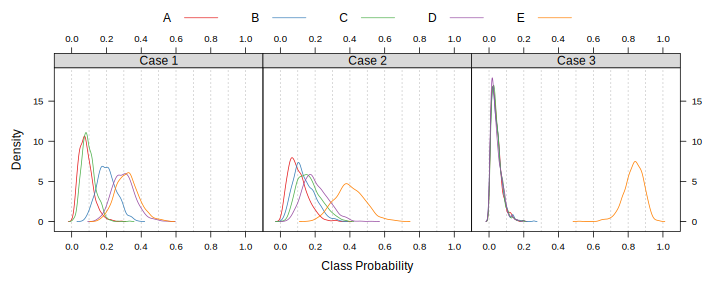
\includegraphics{ch1_prez_files/figure-beamer/unnamed-chunk-2-1.pdf}
\end{frame}

\begin{frame}{What can R do? - Estimate RIC}
\protect\hypertarget{what-can-r-do---estimate-ric}{}
\begin{longtable}[]{@{}llrrr@{}}
\toprule
genhz & variable & pct10 & median & pct90 \\
\midrule
\endhead
A & clay & 13 & 16 & 22 \\
BAt & clay & 16 & 19 & 25 \\
Bt1 & clay & 18 & 24 & 32 \\
Bt2 & clay & 22 & 30 & 44 \\
Cr & clay & 15 & 15 & 15 \\
A & phfield & 6 & 6 & 7 \\
BAt & phfield & 5 & 6 & 6 \\
Bt1 & phfield & 5 & 6 & 7 \\
\bottomrule
\end{longtable}
\end{frame}

\begin{frame}{What can R do? - etc\ldots{}}
\protect\hypertarget{what-can-r-do---etc}{}
\begin{itemize}
\tightlist
\item
  Query and import data from NASIS or SDA
\item
  Develop reports, websites, presentations
\item
  Construct a sampling plan
\item
  Develop pedotransfer functions (e.g.~NASIS calculations)
\item
  Digital soil mapping
\end{itemize}
\end{frame}

\begin{frame}{RStudio - Integrated Development Environment}
\protect\hypertarget{rstudio---integrated-development-environment}{}
\includegraphics[width=0.8\textwidth,height=\textheight]{figure/ch1_rstudio2.png}
\end{frame}

\begin{frame}[fragile]{Rcmdr (R Commander): A Graphical User Interface
for R}
\protect\hypertarget{rcmdr-r-commander-a-graphical-user-interface-for-r}{}
\href{http://gchang.people.ysu.edu/r/R_Instructions.html}{Rcmdr
Tutorials by Andy Chang \& G. Jay Kerns}

\begin{Shaded}
\begin{Highlighting}[]
\FunctionTok{install.packages}\NormalTok{(Rcmdr)}
\FunctionTok{library}\NormalTok{(Rcmdr)}
\end{Highlighting}
\end{Shaded}

\includegraphics[width=0.6\textwidth,height=\textheight]{figure/ch1_rcmdr.png}
\end{frame}

\begin{frame}{Discussion}
\protect\hypertarget{discussion}{}
\begin{enumerate}
\tightlist
\item
  Can you think of a situation where an existing hypothesis or
  convientional wisdom was not repeatable?
\end{enumerate}
\end{frame}

\begin{frame}{(Free) R Learning Resources}
\protect\hypertarget{free-r-learning-resources}{}
\begin{itemize}
\tightlist
\item
  Introductory R Books

  \begin{itemize}
  \tightlist
  \item
    \href{https://r4ds.had.co.nz/index.html}{R for Data Science}
  \item
    \href{https://rstudio.com/resources/cheatsheets/}{RStudio
    Cheatsheets}
  \item
    \href{https://www.statmethods.net/}{Quick-R}
  \end{itemize}
\item
  Advanced DSM R Books

  \begin{itemize}
  \tightlist
  \item
    \href{https://envirometrix.github.io/PredictiveSoilMapping/}{Predictive
    Soil Mapping with R}
  \item
    \href{http://www.springer.com/us/book/9783319443256}{Using R for
    Digital Soil Mapping (not free)}
  \item
    \href{https://github.com/AlexandreWadoux/soilspec}{Soil Spectral
    Inference with R (not free)}
  \end{itemize}
\item
  Soil Science R Tutorials

  \begin{itemize}
  \tightlist
  \item
    \href{http://ncss-tech.github.io/AQP/}{aqp and soilDB tutorials}
  \item
    \href{https://www.isric.org/utilise/capacity-building/training-courses\#examplecourses}{ISRIC
    World Soil Information Example Training Courses}
  \item
    \href{https://www.youtube.com/channel/UCNi1XYjdXWF9eAjvG40KqWg}{ISRIC
    World Soil Information YouTube Channel}
  \item
    \href{https://www.neonscience.org/resources/learning-hub/tutorials}{NEON
    Tutorials}
  \item
    \href{https://pierreroudier.github.io/teaching/index.html}{Pierre
    Roudier}
  \end{itemize}
\end{itemize}
\end{frame}

\begin{frame}
\hypertarget{refs}{}
\begin{CSLReferences}{1}{0}
\leavevmode\hypertarget{ref-arnold1991}{}%
Arnold, R. W., and L. P. Wilding. 1991. {``The {Need} to {Quantify}
{Spatial} {Variability}.''} In \emph{{SSSA} {Special} {Publications}},
edited by M. J. Mausbach and L. P. Wilding, 1--8. Madison, WI, USA: Soil
Science Society of America.
\url{https://doi.org/10.2136/sssaspecpub28.c1}.

\leavevmode\hypertarget{ref-brevik2016}{}%
Brevik, Eric C., Jeffrey A. Homburg, Bradley A. Miller, Thomas E.
Fenton, James A. Doolittle, and Samuel J. Indorante. 2016. {``Selected
Highlights in American Soil Science History from the 1980s to the
Mid-2010s.''} \emph{{CATENA}} 146 (November): 128--46.
\url{https://doi.org/10.1016/j.catena.2016.06.021}.

\leavevmode\hypertarget{ref-chaney2016}{}%
Chaney, Nathaniel W., Eric F. Wood, Alexander B. McBratney, Jonathan W.
Hempel, Travis W. Nauman, Colby W. Brungard, and Nathan P. Odgers. 2016.
{``{POLARIS}: A 30-Meter Probabilistic Soil Series Map of the Contiguous
United States.''} \emph{Geoderma} 274: 54--67.
\url{https://doi.org/10.1016/j.geoderma.2016.03.025}.

\leavevmode\hypertarget{ref-hennemann2004}{}%
Hennemann, G R, and D G Rossiter. 2004. {``Training Needs for the Next
Generation of Soil Surveyors.''} In \emph{International Conference on
Innovative Techniques in Soil Survey, Cha'am, Thailand, 21-26 March
2004}, 22--26. Cha-Am, Thailand: Land Development Department.
\url{http://www.css.cornell.edu/faculty/dgr2/Docs/ChaAm/ChaAmKeynoteHennemann.pdf}.

\leavevmode\hypertarget{ref-kempen2012}{}%
Kempen, Bas, Dick J. Brus, Jetse J. Stoorvogel, Gerard B. M. Heuvelink,
and Folkert de Vries. 2012. {``Efficiency Comparison of Conventional and
Digital Soil Mapping for Updating Soil Maps.''} \emph{Soil Science
Society of America Journal} 76 (6): 2097--2115.
https://doi.org/\url{https://doi.org/10.2136/sssaj2011.0424}.

\leavevmode\hypertarget{ref-macmillan2007}{}%
MacMillan, Robert A., David E. Moon, and Ray A. Coupé. 2007.
{``Automated Predictive Ecological Mapping in a Forest Region of b.c.,
Canada, 2001--2005.''} \emph{Geoderma} 140 (4): 353--73.
\url{https://doi.org/10.1016/j.geoderma.2007.04.027}.

\leavevmode\hypertarget{ref-mausbach2003}{}%
Mausbach, M. J. 2003. {``The Importance of Statistical Documentation -
Keeping Soil Survey Information Relevant in the 21st Century.''} In
\emph{2003 National Cooperative Soil Survey Conference}, 3--6. Plymouth,
Massachusetts: National Cooperative Soil Survey.
\url{https://www.nrcs.usda.gov/Internet/FSE_DOCUMENTS/nrcs142p2_051833.pdf}.

\leavevmode\hypertarget{ref-maynard2019}{}%
Maynard, Jonathan J., Travis W. Nauman, Shawn W. Salley, Brandon T.
Bestelmeyer, Michael C. Duniway, Curtis J. Talbot, and Joel R. Brown.
2019. {``Digital {Mapping} of {Ecological} {Land} {Units} Using a
{Nationally} {Scalable} {Modeling} {Framework}.''} \emph{Soil Science
Society of America Journal} 83 (3): 666--66.
\url{https://doi.org/10.2136/sssaj2018.09.0346}.

\leavevmode\hypertarget{ref-ramcharan2018}{}%
Ramcharan, Amanda, Tomislav Hengl, Travis Nauman, Colby Brungard, Sharon
Waltman, Skye Wills, and James Thompson. 2018. {``Soil Property and
Class Maps of the Conterminous United States at 100-Meter Spatial
Resolution.''} \emph{Soil Science Society of America Journal} 82 (1):
186--201.
https://doi.org/\url{https://doi.org/10.2136/sssaj2017.04.0122}.

\end{CSLReferences}
\end{frame}

\end{document}
